\documentclass{article}
\usepackage{graphicx}
\usepackage{color}
\title{Prelim Outline (ROUGH)}
\author{Shivesh Pathak}

\begin{document}
\maketitle

\color{red} Red \color{black} is incomplete preliminary work.
\color{blue} Blue \color{black} is work for the future.

\section{Motivation/Background}
\begin{enumerate}
\item People want to construct an accurate low-energy model Hamiltonian for the cuprates.
\item Hole doped cuprates have been studied for a long time and have many degrees of freedom: O p and Cu d orbitals both play roles.
\item Electron doped cuprates are less studied and we believe they are simpler since only the Cu d orbitals play a major role.
\item We plan on building an low-energy model for the electron doped cuprate SrCuO$_2$ using a density-matrix downfolding method and accurate many-body QMC calculations.
\end{enumerate}

\section{Preliminary SCF calculations}
\subsection{Undoped (x=0)}
\begin{enumerate}
\item We did eight unit cell PBE0 calculations to calculate the energies of states with singly occupied Cu d$_{x^2-y^2}$ orbitals but with different spin textures.

\item We mapped these states onto spin-1/2 local moment states and used to fit to an AFM Heisenberg model:
$$H_m = J\sum_{ij} \frac{1}{2} \vec{S_i}\cdot\vec{S_j} $$ 

\item The results of this fitting on seven different spin textures yields good results for two different basis sets (BFD Cutoff, BFD PBC 0.2)

\item The high $R^2$ values of these fits indicate that a simple AFM Heisenberg model should be sufficient to capture the low-energy behavior of the undoped cuprates.
\end{enumerate}

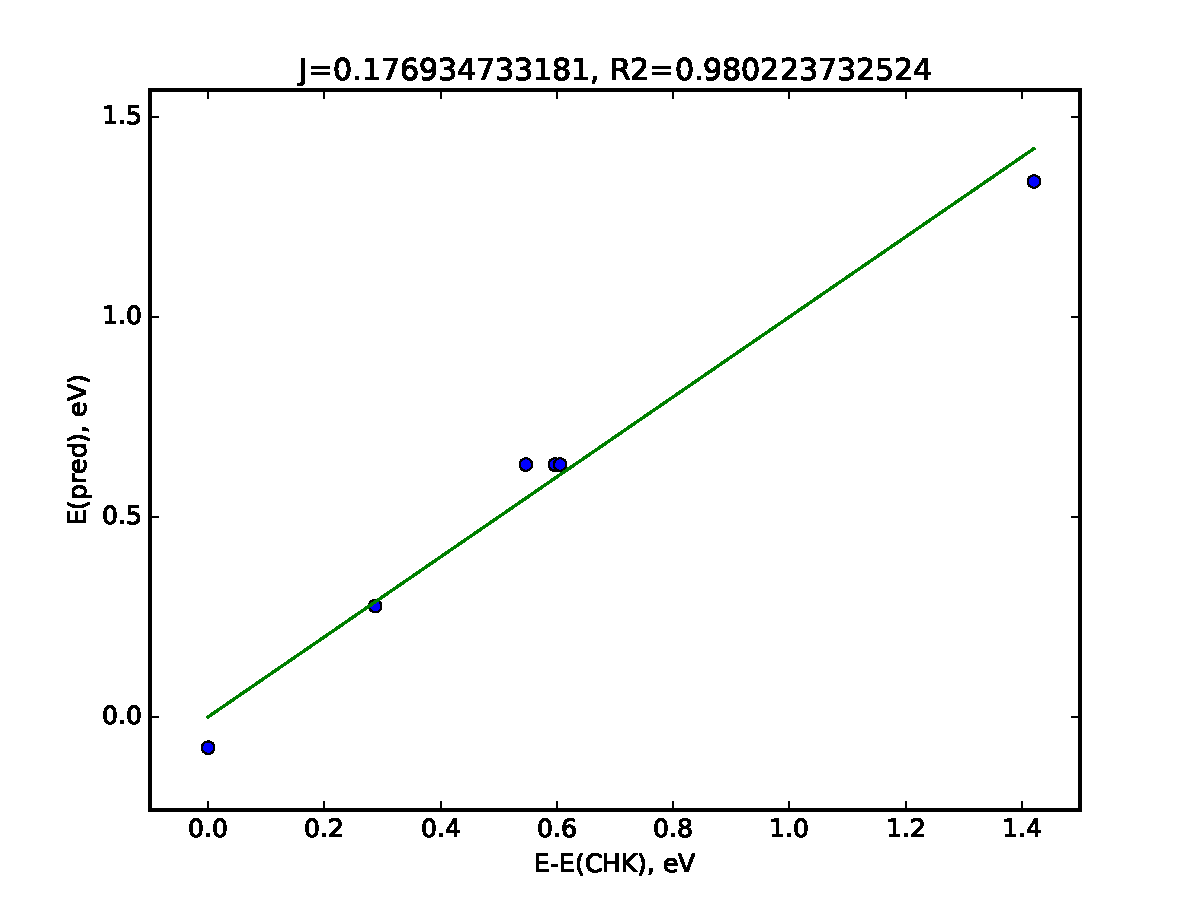
\includegraphics[width=0.5\textwidth]{../undoped/PBE0_8/J_fit_naive.pdf}
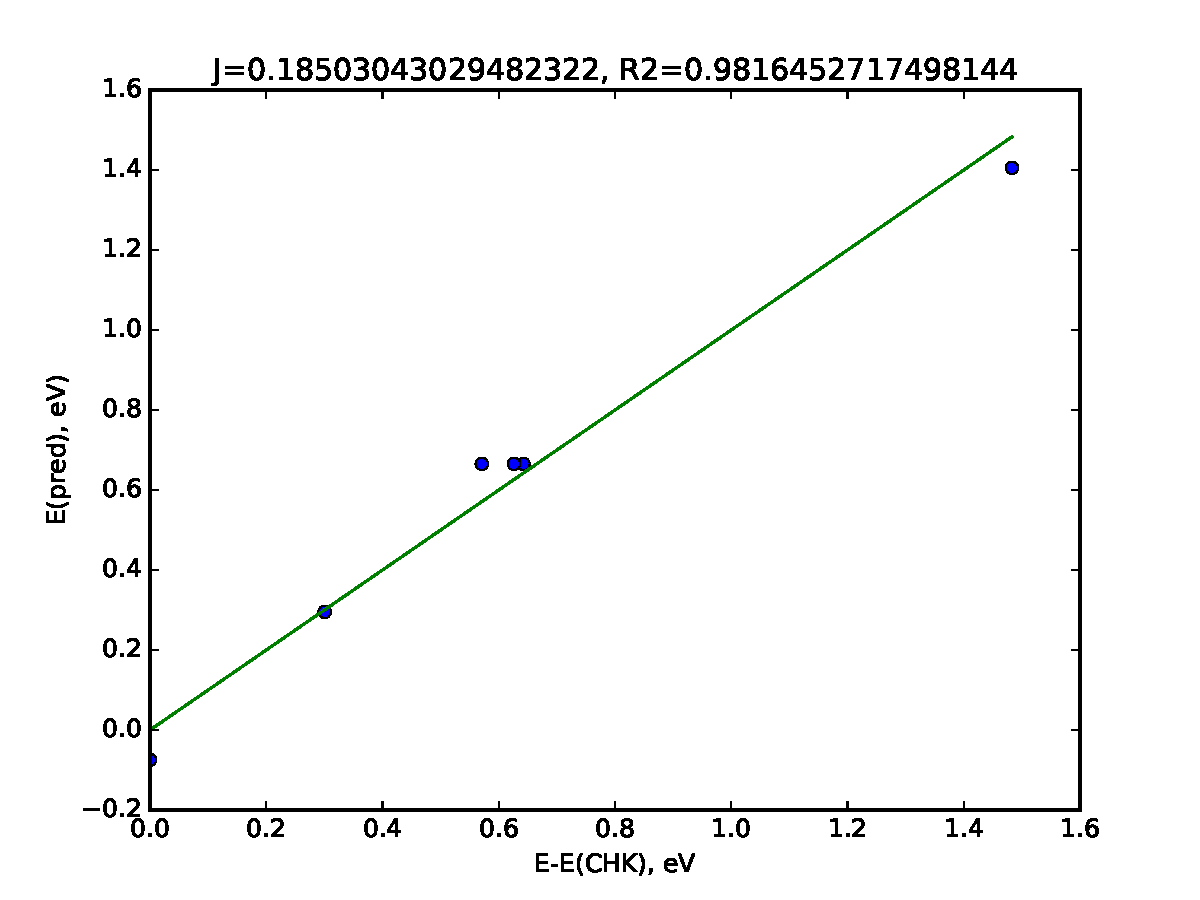
\includegraphics[width=0.5\textwidth]{../undoped/PBE0_8/J_fit_naive_BFD0p2.pdf}

\subsection{Overdoped (x=0.25)}
\begin{enumerate}
\item We similarly did seventeen x=0.25 doped calculations in PBE0, from we got four low energy states. Here low-energy is defined as states with energy less than 0.3 eV from the lowest energy state we had, a collinear doped state.

\item We then used the band structures and energies of these four low energy states to fit to a naive model with $t, t^\prime, K, J$ parameters: NN-hopping, NNN-hopping, NN-Kondo term, and NN-Heisenberg-AFM term

$$H_m =  -t\sum_{\langle i, j \rangle, \sigma} (c_{i\sigma} ^\dagger c_{j\sigma} + h.c.) + 
t^\prime\sum_{\langle\langle i, j \rangle\rangle, \sigma} (c_{i\sigma} ^\dagger c_{j\sigma} + h.c.) + $$ 
$$K \sum_{\langle i, j \rangle} \vec{S_i} \cdot c_{j\alpha}^\dagger \vec{\sigma}_{\alpha \beta} c_{j\beta} + J\sum_{ij} \frac{1}{2} \vec{S_i}\cdot\vec{S_j} $$ 

\item The presence of $t, t^\prime$ parameters were necessary to get the correct curvature of bands near the Fermi level, and the $K, J$ parameters were necessary to get both the spacing between bands (K) and the total energies (K,J). 

\item We map each of the PBE0 states into the model Hilbert space by breaking the occupied bands into a) fully occupied and b) partially occupied. The orbitals from a) then build a spin density that defines the variables $\vec{S_i}$ and the orbitals from b) define the variables $c_i^\dagger$.

\item We can therefore create a single body  Hamiltonian where we treat the spins $\vec{S_i}$ as a fixed background upon which the itenerant $c_i^\dagger$ electrons can move. We can solve this model Hamiltonian and fit to the PBE0 band structure, and also compare the total energy of the model to the PBE0 total energy.

\item We use a prior where $J$ is held as the undoped value. This is because in a metallic/superconducting doped state, there are charge fluctuations locally. Therefore we expect that on average the total charge locally between nearest neighbors will be the undoped value, and since the Heisenberg model only has local coupling we don't imagine $J$ should change too much.

\item Since we are fitting to two different quantities (total energy and band structure) we used a Pareto efficiency analysis to get the best balance between a fit to total energy and a fit to band structure. The cost function is shown below, and $w_E$ varies in the plot shown even lower for the two different basis sets from before.

$$Cost = w_E|E_m - E_{PBE0}|^2 + \sum_{|k|\le k_F} |e_{m,k} - e_{PBE0,k}|^2$$
 
\item We find that the most efficient point is at the blue square on the Pareto plot. Below we plot the fit to the band structure and comparison of the model and PBE0 total energies. 

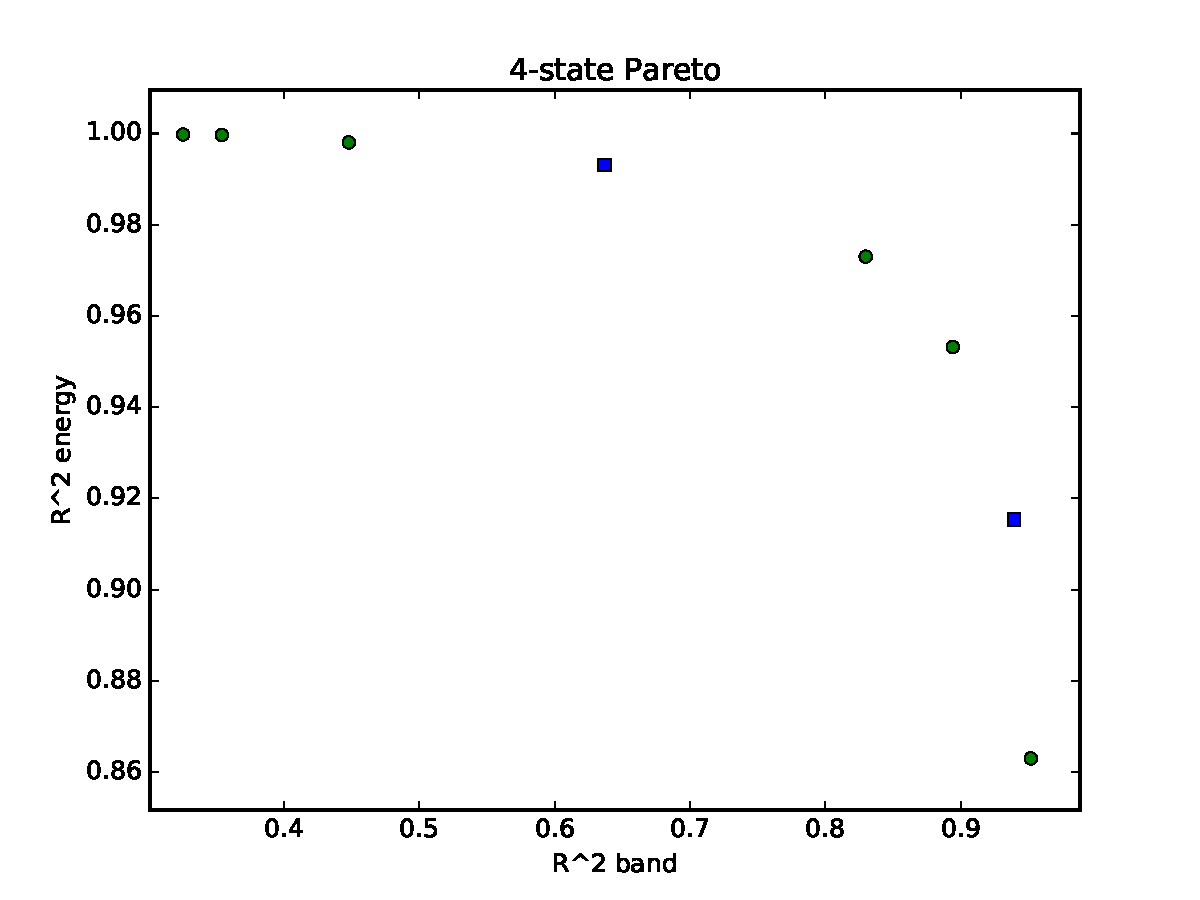
\includegraphics[width=0.5\textwidth]{../doped_fv/PBE0_8/tb_fit/pareto4.pdf}
\linebreak
\color{red} Need to include plot for PBC 0.2 basis set.

\color{black}

\item For the BFD cutoff basis set we get the parameter values $t,t^\prime,K,J=  1.04, 0.53, -0.15, 0.18 eV$

\item The two basis sets do not agree quantitatively, but this isn't too unexpected because it's such a rough fitting method, but qualitatively they do: AFM J, FM K, repulsive NNN hopping, attractive NN hopping.

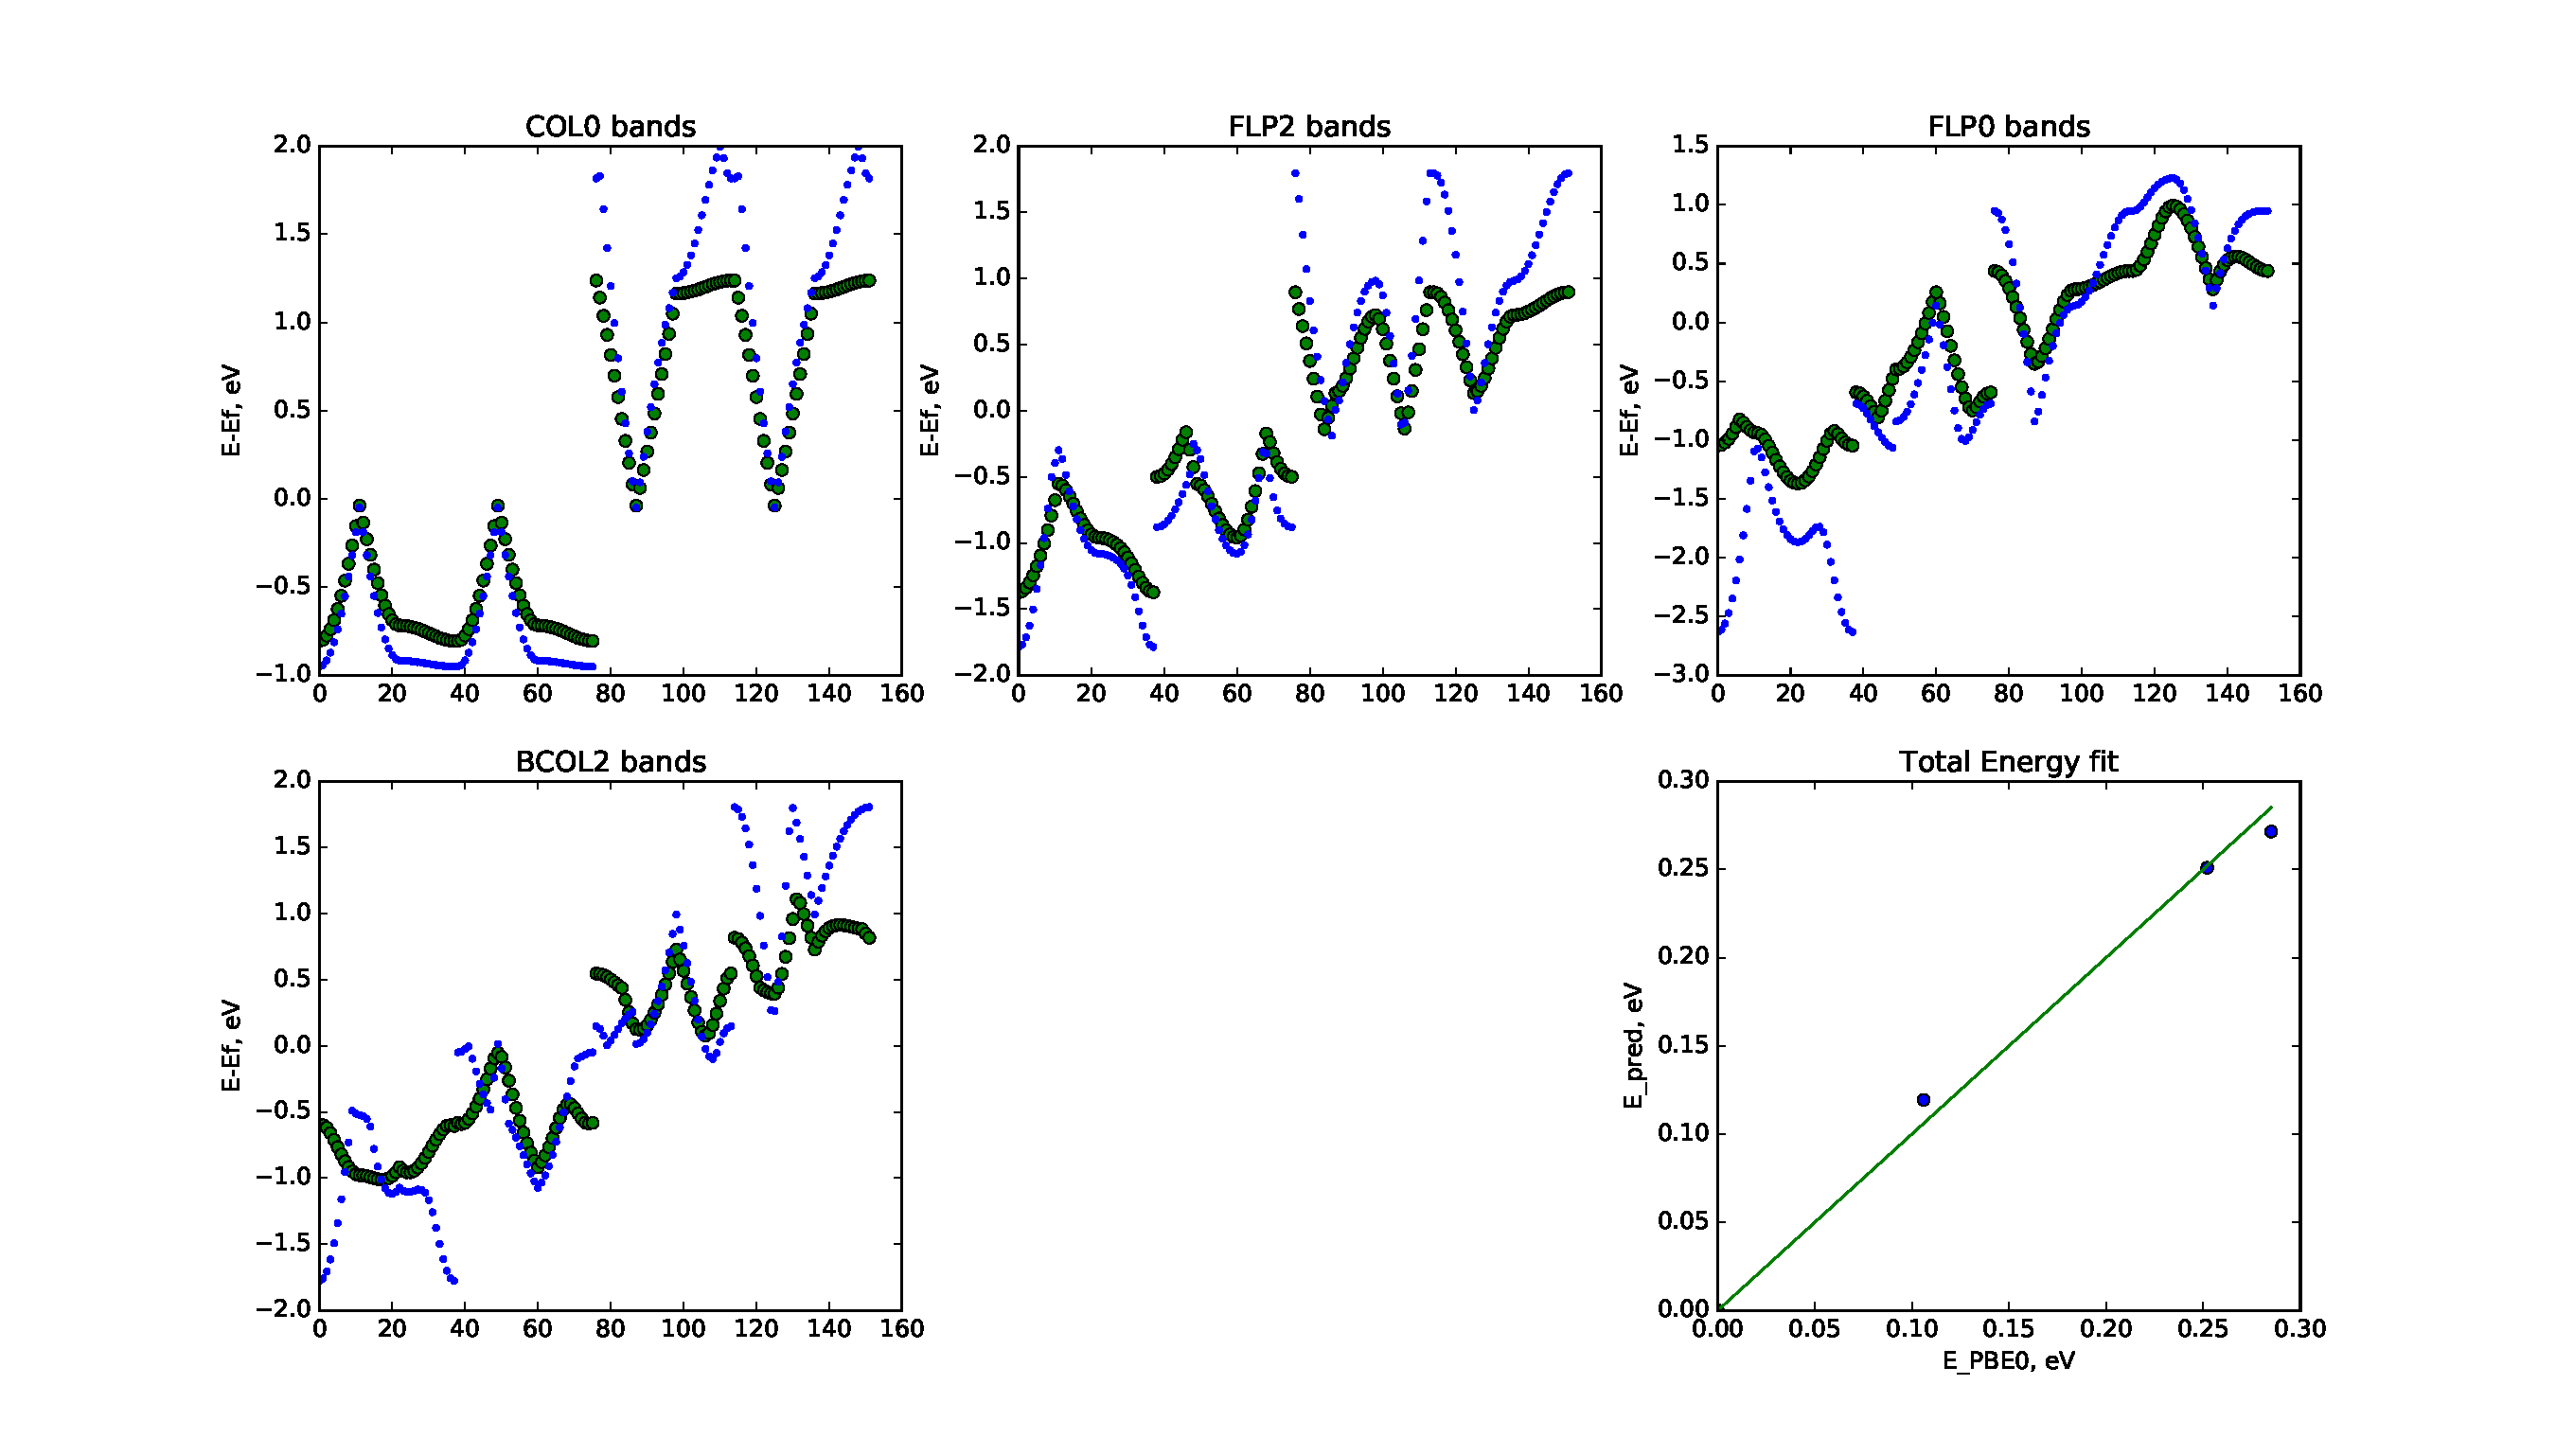
\includegraphics[width=\textwidth]{../doped_fv/PBE0_8/tb_fit/pareto4_high.pdf}
\color{red} Need to include plot for PBC 0.2 basis set.
\end{enumerate}

\subsection{Optimally doped (x=0.125)}
\color{red} Need to do these calculations, but analysis is identical to above.

\color{black}
\section{Density matrix downfolding (DMD) calculations}
\subsection{Basis}

\begin{enumerate}
\item In order to do our DMD calculations we need a single particle basis to evaluate the density matrix on.  We use intrinsic atomic orbitals (IAOs) as our one particle basis. Justification for this choice is provided below.

\item \textbf{Undoped (x=0)}]
\begin{enumerate}
\item Shown below are the occupations of different IAOs for the checkerboard spin texture for the BFD Cutoff and BFD PBC 0.2 basis sets. 

\item Clearly the IAOs show that the primary variation between occupation is in the $3d_{x^2-y^2}$ orbital, namely the spin changes from site to site. The oxygen orbitals do not play a significant role, indicating that this basis captures the qualitative features that we expect from the undoped state.

\item Another important feature is that for each copper atom there are TWO $3d_{x^2-y^2}$ IAOs: one for the occupied spin and one of the unoccupied spin.

\end{enumerate}
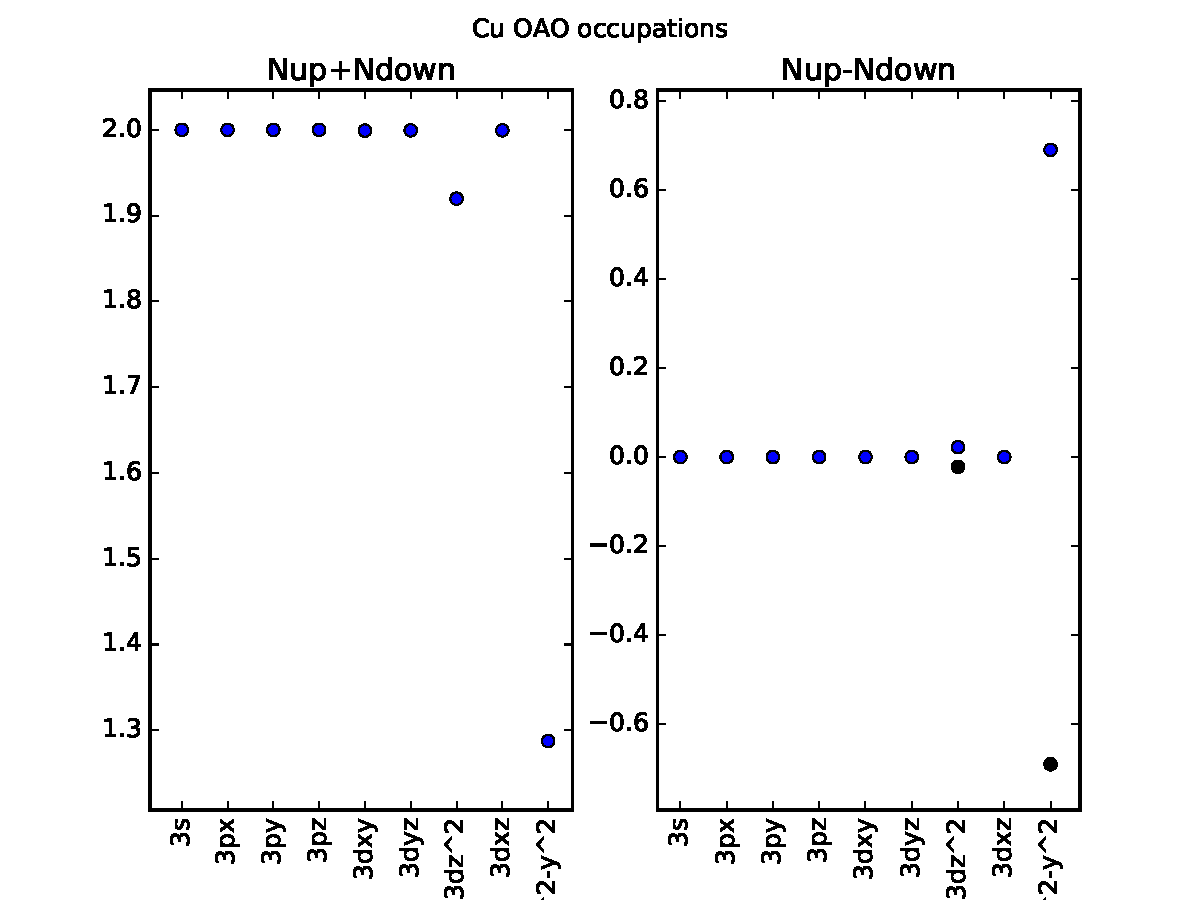
\includegraphics[width=0.5\textwidth]{../undoped/PBE0_8/CHK/dens_iao2_cu.pdf}
\linebreak
\color{red} Need to include plot for PBC 0.2 basis set.

\color{black}
\item \textbf{Overdoped (x=0.25)}
\begin{enumerate}
\item For the doped calculation, we did the same IAO analysis as for the x=0 case. We found that again the $3d_{x^2-y^2}$ orbital has the primary variation in occupation. 

\item Unlike the x=0 case, once doped the occupation number changes as well as the spin. Below is shown the difference in occupation of the spin-down and spin-up $3d_{x^2-y^2}$ orbitals of the doped collinear state compared to the UNDOPED collinear state. 

\item We see that the occupation of the dominant primary channel does not vary, and we can therefore attribute those orbitals to the fixed magnetic moments, and the secondary spin channel does vary and we can attribute those orbitals to the itinerant electrons.

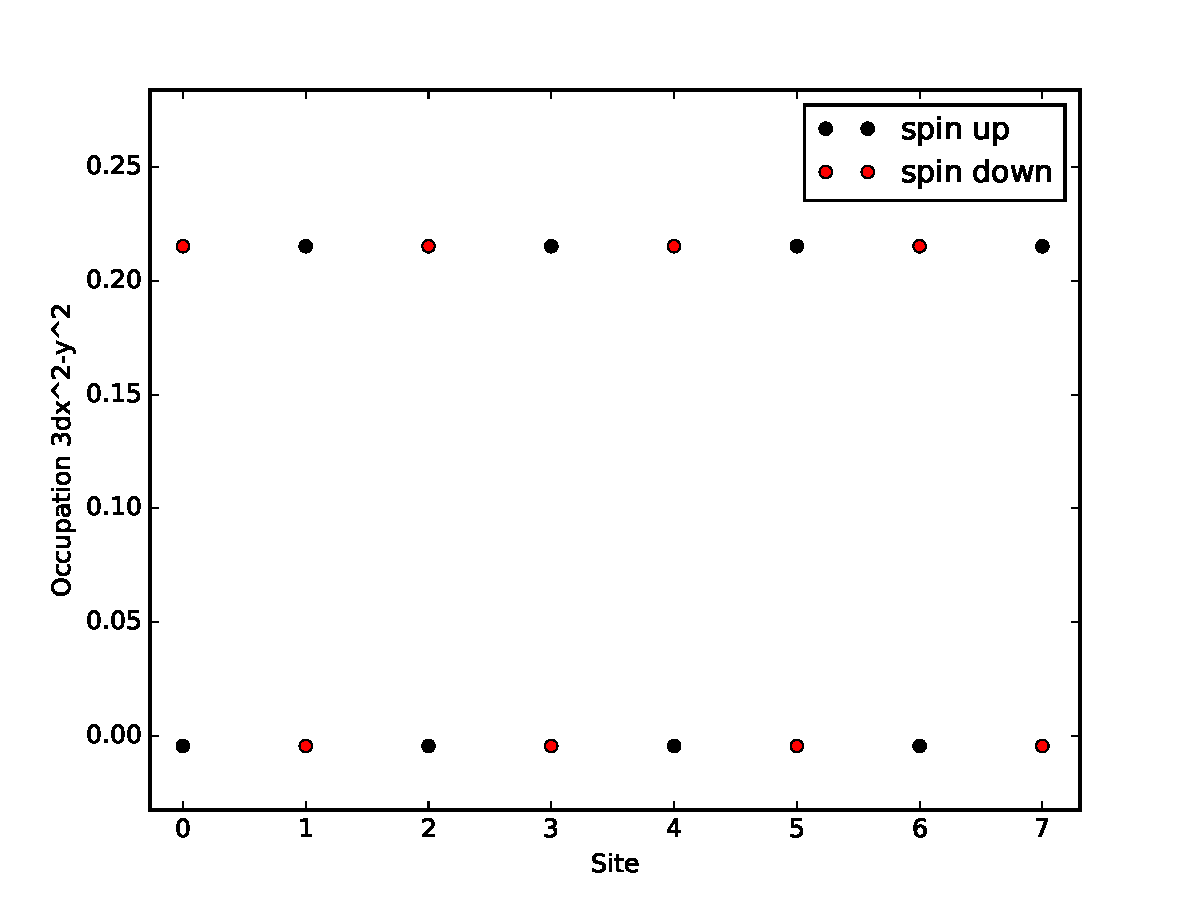
\includegraphics[width=0.5\textwidth]{../doped_fv/PBE0_8/COL0/iao/sub_occd.pdf}
\linebreak
\color{red} Need to include plot for PBC 0.2 basis set.

\color{black}
\item Therefore we see that the basis elements we will be constructing our DM out of are the two different $3d_{x^2-y^2}$ IAOs: the orbital corresponding to the primary spin channel will be used to calculate DM elements of the fixed spin moments $\vec{S_i}$ and the secondary spin channel IAO will be used to calculate DM elements of the itinerant electrons $c_i^\dagger$
\end{enumerate}

\item \textbf{Optimally doped (x=0.125)}
\color{red} Need to do this, should be identical analysis to x=0.25.
\end{enumerate}

\color{blue}
\subsection{States}
\begin{enumerate}
\item \textbf{Undoped (x=0)} For the undoped calculations, we have seven different spin textures. We can just use these for the model fitting since we will be fitting to a single parameter, $J$.

\item \textbf{Overdoped (x=0.25)}
\begin{enumerate}
\item We have four low energy states for x=0.25. We will use these four states, as well as states that are singles (maybe double) excitations above these four states. Only states with energy lower than our cutoff will be used.
\item We can also take linear combinations of states with singles and double excitations. This can help us generate many more states and also increase our fitting efficiency since we can then make use of parameter derivatives w.r.t the determinant coefficients.
\end{enumerate}

\color{red}
\item \textbf{Optimally doped (x=0.125)}
\begin{enumerate}
\item Need to do this, should be similar.
\end{enumerate}
\color{blue}
\end{enumerate}

\subsection{K-points}
\begin{enumerate}
\item \textbf{Undoped (x=0)} For the undoped calculations, a $\Gamma$ point calculation should be sufficient to resolve any finite size effects because we have a large unit cell for calculation and the system is strongly insulating.

\item \textbf{Doped (x=0.25, 0.125)}
\begin{enumerate}
\item For the doped calculations our first goal will be to do calculations just on the $\Gamma$ point, since this should give us a good sense of whether the model we are interested in makes sense or not.

\item We can consider doing other k-point (twist boundary) calculations if we think that the finite size errors on the calculations at a single twist are too large.
\end{enumerate}
\end{enumerate}

\subsection{QMC workflow}
for x=0, 0.125, 0.25 \\
\indent for k-points from section (3) \\ 
\indent \indent for states from section (2) \\
\indent \indent \indent Take lowest energy Slater det, variance optimize Jastrow;\\
\indent \indent \indent use this Jastrow for all following calculations
\\

\indent \indent \indent Calculate 1/2-RDM and quantities for parameter derivative fitting \\ 
\indent \indent \indent using FN-DMC for basis elements in section (1)\\

\noindent Conduct fitting to $t,t^\prime, K,J$ model using DMD method with parameter derivative fitting. \\

\noindent Alter k-points, states from sections (3) and (2) as necessary for calculation.  



\end{document}